\documentclass{beamer}
\usepackage{Stil}
\begin{document}
\title[Freie Netzer]{Freifunk-MYK}
\subtitle[Freifunk-MYK]{Freie Netze}
\author[Freifunk-MYK]{Norbert Härig, Michael Lambert}
\date{\today\\\vspace{0.5cm} 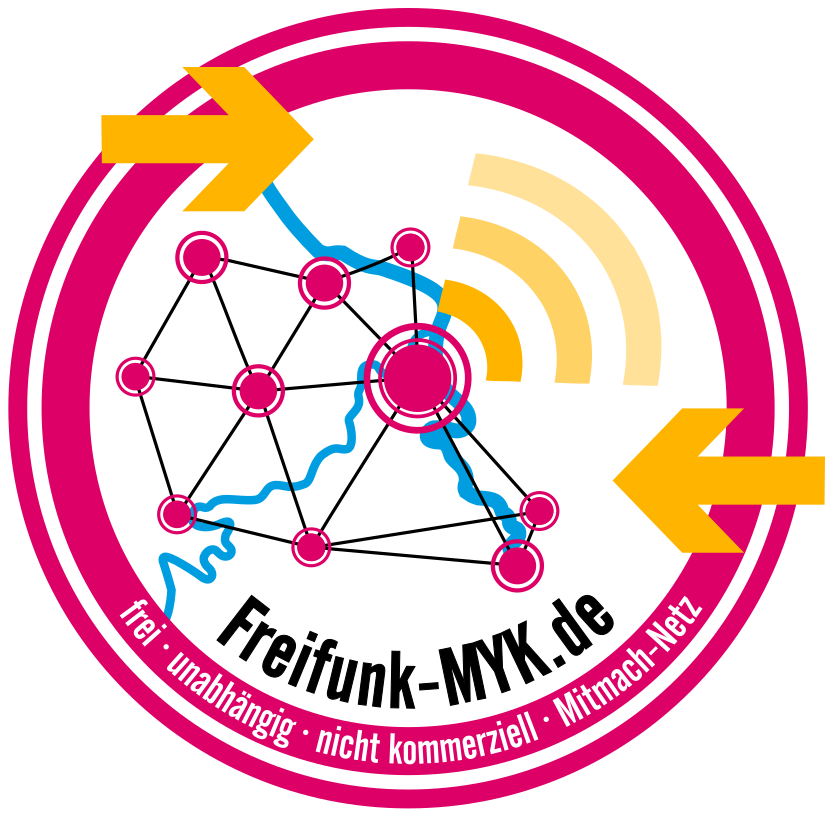
\includegraphics[scale=0.1]{Bilder/Logo.png}}
\institute{}

\begin{frame}
\titlepage	
\end{frame}
\begin{frame}{Inhaltsverzeichnis}
	\tableofcontents
\end{frame}
\section{Kapitel 1}
\begin{frame}{Titel der ersten Folie}
\begin{itemize}
	\item Punkt 1
	\item Punkt 2
\end{itemize}
\end{frame}
\section{Kapitel 2}
\begin{frame}{Titel der zweiten Folie}
	\begin{itemize}
		\item Punkt 1
		\item Punkt 2
	\end{itemize}
\end{frame}


% und hier beginnt die Präsentation
\begin{frame}{Referenten}
\begin{itemize}
	\item Norbert Härig
	\begin{itemize}
		\item Brohl
		\item Student
		\item Freifunker seit 2014
	\end{itemize}
	\item Michael Lambert
	\begin{itemize}
		\item Sinzig
		\item EDV-Koordinator Schulen im Kreis Ahrweiler
		\item Freifunker seit 2016
	\end{itemize}
\end{itemize}
\end{frame}

\begin{frame}{Freie Netzwerke - Wozu?}
\begin{itemize}
	\item Die Informations- und Kommunikationsfreiheit im Internet wird zunehmend eingeschränkt.
	\item Trotz des Slogans "Internet für alle" gibt es Anzeichen einer sich verfestigenden digitalen Kluft - ärmere, weniger technisch versierte und ältere Menschen nehmen wenig oder gar nicht am sogenannten Informationszeitalter teil.
	\item Besonders für Flüchtlinge wertvoll zur Kontaktaufnahme mit der Heimat und als Informationsquelle (Ärzte, Infos über die Stadt, ...).
	\item In dünn besiedelten und strukturschwachen Gebieten (“areas of market failure”) werden keine (bezahlbaren) Breitbandanschlüsse angeboten.
	\item Besser ein Netz, das der Gemeinschaft gehört als eins, das von wenigen Großkonzernen kontrolliert wird.
	
\end{itemize}
\end{frame}

\begin{frame}{WLAN - Wozu?}
WLAN vs. Mobilfunk
\begin{itemize}

\item Geringe Abdeckung in ländlichen Regionen
\item Je nach Tarif teuer / Limit
\item Geräte ohne SIM
\end{itemize}
\end{frame}

\end{document}
